\documentclass[../../dissertation.tex]{subfiles}
\begin{document}

As was seen in section \ref{sec:chap3Contwalk}, the unitary evolution operator
of this model is defined as
\begin{equation}
        U(t) = e^{-iHt} = e^{i(\gamma L)t} = e^{i\gamma(A-D)t}.
\end{equation}
Considering a regular graph, this operator can be rewritten as 
\begin{equation}
	U(t) = \phi(t) e^{i\gamma(A)t},
\end{equation}
where $\phi(t)$ is a global phase and $A$ is the adjacency matrix associated
with the graph.\par

In this section, the study will focus on the circuit implementation of this walk in a
cycle graph, where the associated adjacency matrix will be defined using a circulant matrix. The motivation behind this choice was that the circulant graph class can be easily diagonalized with the quantum Fourier transform, which means it has a straightforward implementation in Qiskit.\par The class of circulant
graphs is defined by a circulant adjacency matrix such that
\begin{equation}
A = 
	\begin{pmatrix}
		c_0&c_{N-1}& \cdots&c_3&c_2 \\
		c_1&c_0& c_{N-1}& &c_{3} \\
		\vdots & c_1 & c_0 &\ddots & \vdots\\
		c_{N-2}& & \ddots&\ddots &c_{N-1}\\
		c_{N-1} & c_{N-2} & \cdots & c_1 & c_0\\
	\end{pmatrix},
\label{eq:adjCirculant}
\end{equation}
where $c_k = 1$ if the vertices are connected, and $0$ otherwise.
In order to generate the proper circulant graphs, restrictions on this matrix
are in order. Firstly, $c_0=0$, since self-loops are not part of the structure.
Secondly, the matrix must be symmetric, therefore $c_{n-j} = c_j$.\par

These matrices can be fully described by their first columns 
\begin{equation}
	v_1 = [c_{0},c_{1}, \cdots, c_{N-2}, c_{N-1}]^T ,
\end{equation}
with a discrete convolution operator performing cyclic permutations of $c$, on
each column, known as the \textit{deque} operator. For example,
\begin{equation}
	D v_1 = [c_{N-1}, c_{0}, \cdots, c_{N-3}, c_{N-2}]^T = v_2.
\end{equation}
More specifically, for the cycle case
\begin{equation}
	D v_1 = D [0, 1 ,0 , \cdots, 0, 1]^T =[1, 0, 1, 0, \cdots, 0, 0]^T = v_2.
\end{equation}
The eigenvalues of a circulant matrix are given by
\begin{equation}
\lambda_p = c_0 + \sum_{q=1} c_{N-q} \omega^{pq},
\end{equation}
and the eigenvectors by 
\begin{equation}
\ket{\varphi_p} = \frac{1}{\sqrt{n}} \sum_{q=0}^{n-1} \omega^{pq}.
\end{equation}
This given, it is possible to construct an operator that diagonalizes the
circulant matrix through the eigenvectors, which is useful for constructing the
circuit. For this purpose, the quantum Fourier transform can be used. It is
defined by 
\begin{equation}
F = \frac{1}{\sqrt{N}} \sum_{p,q} \omega^{pq} \ket{p}\bra{q},
\end{equation}
and further reading can be done in appendix \ref{sec:chapQFT}.
The adjacency matrix of a circulant graph is then diagonalized such that
\begin{equation}
    A = F^{\dagger} \Lambda F,
    \label{eq:qiskitContQWAdj}
\end{equation}
where $\Lambda$ is a diagonal operator that encodes the eigenvalues, i.e.
\begin{equation}
\Lambda = \sum_{j} \lambda_j \ket{j}\bra{j}.
\end{equation}\par
%TODO: Mostrar o raciocinio da algebra.
The unitary operator of the walk can then be rewritten as
\begin{equation}\label{eq:diagUniOpCont}
    U = F^{\dagger}e^{i\gamma \Lambda t} F,
\end{equation}
where
\begin{equation}
    e^{i\gamma \Lambda t} = \sum_{j} e^{i\gamma \lambda_j t} \ket{j}\bra{j}.
\end{equation}
This representation is very easily translatable to a quantum circuit, as shown in figure \ref{fig:contCircuit}.
\begin{figure}[!h]
	\[ \Qcircuit @C=1.8em @R=1.5em {
	& & {/^{\otimes n}} \qw &\gate{QFT_m}  & \gate{e^{i\gamma\Lambda t}} &  \gate{QFT^{\dagger}_m} &\qw &\qw 
		          } \]
	\centering
	\caption{General circuit for the continuous-time quantum walk.}
	\label{fig:contCircuit}
\end{figure}\par

The circuit can now be constructed making use of the \textit{diagonal} function
provided by Qiskit, which decomposes diagonal operators based on the method
presented in theorem 7 of \cite{shendel06}. The other tool used was the quantum
Fourier transform (QFT) also provided by the Qiskit package. Figure
\ref{fig:contQWCircuitQistkit} shows the implementation of the circuit for
$2^3=8$ graph nodes.
\begin{figure}[!h]
	\centering
	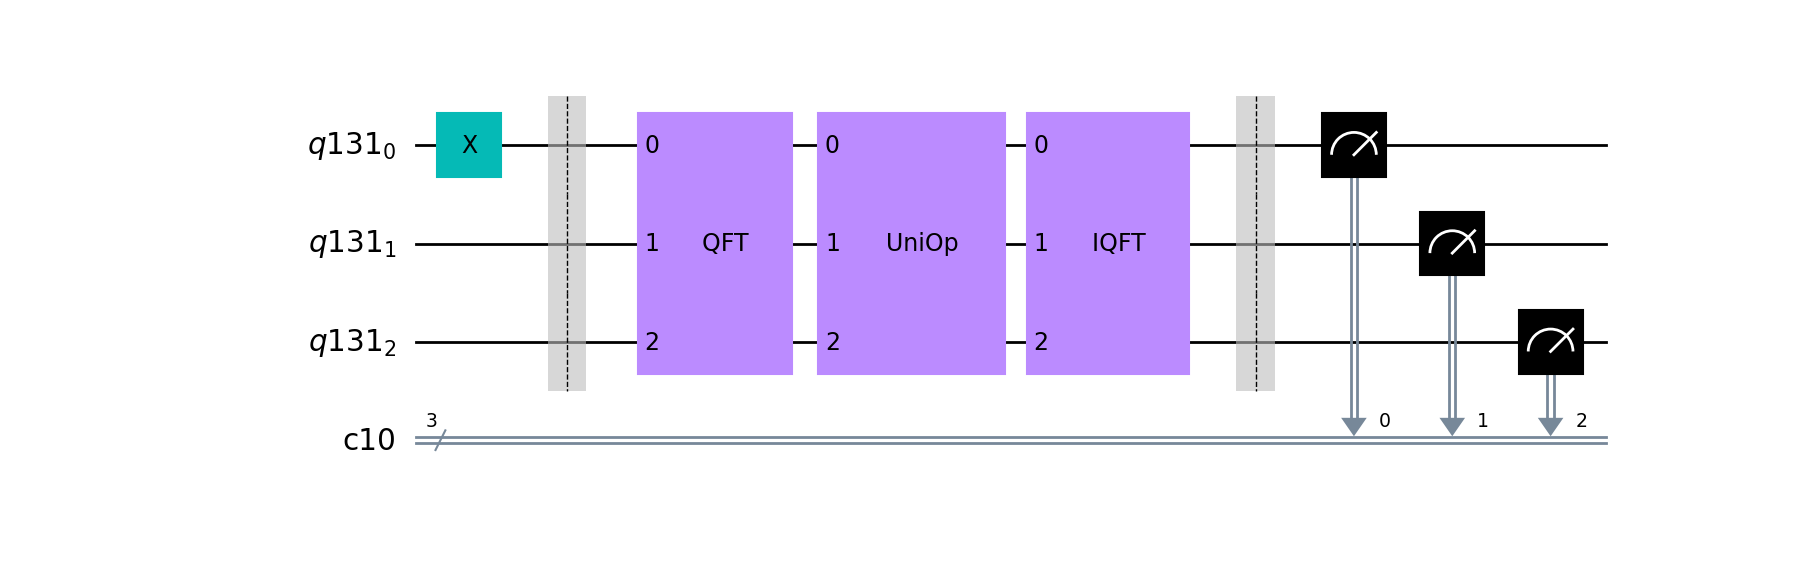
\includegraphics[scale=0.25]{img/Qiskit/ContQuantumWalk/Circuits/circContQW_N3_S1.png}
	\caption{Qiskit circuit for the continuous-time quantum walk, for a line graph of size $N=8$ and initial condition $\ket{\psi_0}=\ket{4}$, for time $t$.} 
	\label{fig:contQWCircuitQistkit}
\end{figure}\par

The quantum Fourier transform circuit, presented in figure
\ref{fig:qftCircuitQiskit}, is well known. The inverse QFT is similarly
constructed by changing the signs of the angles of rotation associated with the QFT.
\begin{figure}[!h]
	\centering
	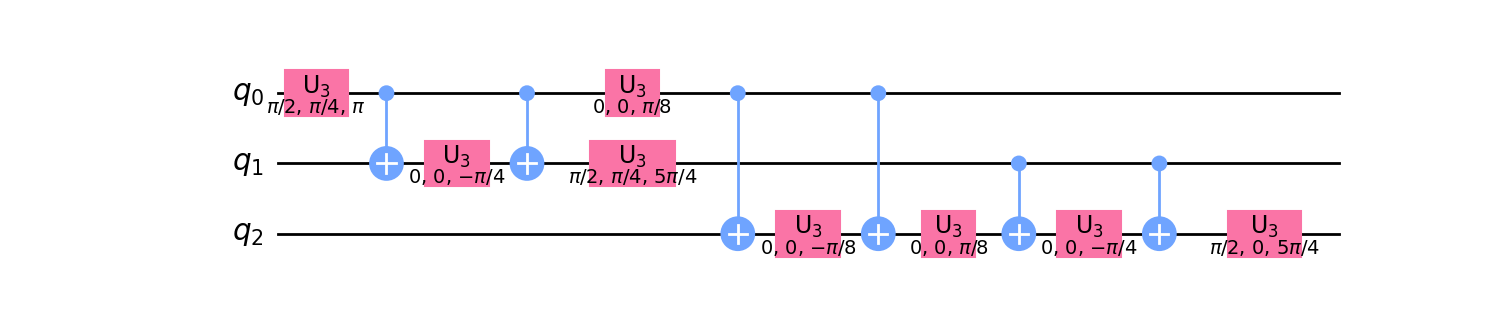
\includegraphics[scale=0.28]{img/Qiskit/ContQuantumWalk/Circuits/circQft_N3_S1.png}
	\caption{Qiskit circuit of the quantum Fourier transform for a line graph of size $N=8$.} 
	\label{fig:qftCircuitQiskit}
\end{figure}\par

The circuit associated with the diagonal operator is shown in figure
\ref{fig:diagCircuitQiskit}. Furthermore equation \eqref{eq:diagUniOpCont} says
that time is simply a constant inside the exponential, which means that the
diagonal operator's circuit will not need extra operations when increasing
time, only when in size. It will simply require different rotations and it will differ in global phase.  This
is an advantage when comparing to previous discrete models,  where each extra
step required another increment and decrement gates.
\begin{figure}[!h]
	\centering
	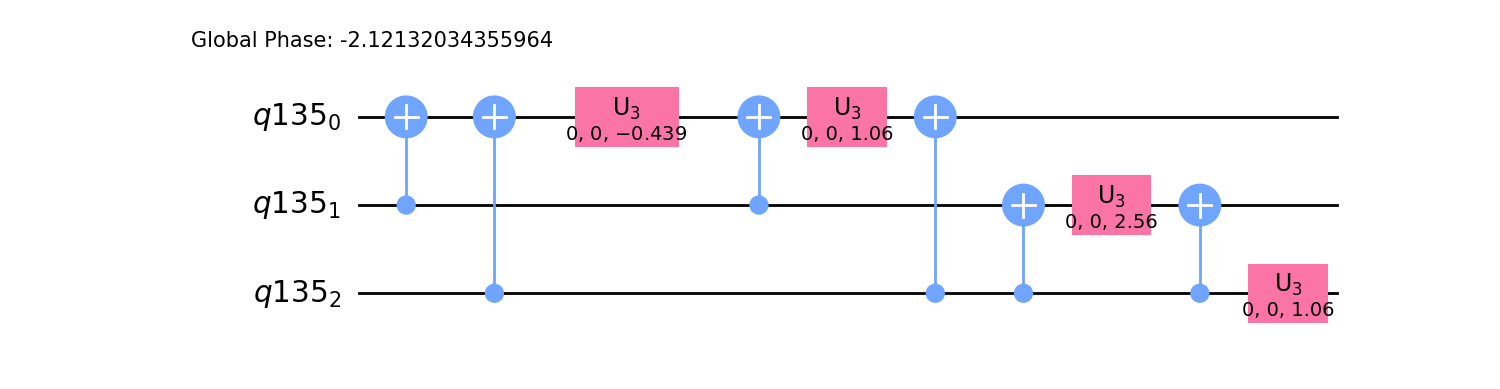
\includegraphics[scale=0.50]{img/Qiskit/ContQuantumWalk/Circuits/circDiag_N3_S1.png}
	\caption{Qiskit circuit of the diagonal operator associated with the adjacency matrix, for a line graph of size $N=8$.}
	\label{fig:diagCircuitQiskit}
\end{figure}\par

Finally, the circuit was measured. The resulting probability distributions
can be seen in figure \ref{fig:contQWQiskitDist}.\par

The dynamics of the walk, when ran on the Toronto backend, is closer to the
simulation than the previous examples. Now, the size of the
circuit does not scale with time, and $29$ CNOT gates were required to implement the walk for $t = 1$, $2$ and $3$. \par
A fidelity of approximately $0.97$ was
achieved for $t=3$. For $t=0, 1, 2$, the respective fidelities were $0.96, 0.90,
0.92$, which are small improvements when compared to the staggered quantum
walk.
\begin{figure}[!h]
	\centering
	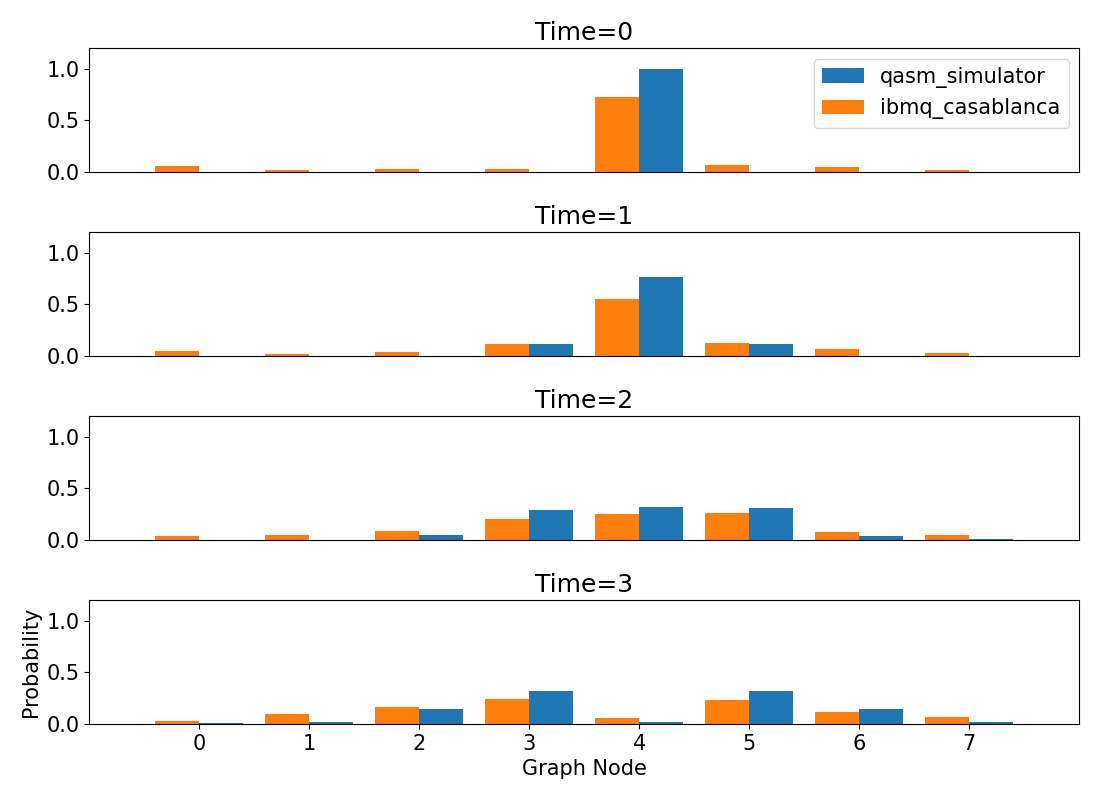
\includegraphics[scale=0.4]{img/Qiskit/ContQuantumWalk/ContQW_N3_S0123.png}
	\caption{Probability distributions of the continuous-time quantum walk for several steps in a line graph of size $N=8$. The blue bar plot represents a circuit run in the QASM simulator, and the orange bar plot on IBM's Toronto backend.} 
	\label{fig:contQWQiskitDist}
\end{figure}
Fidelity also stays relatively constant with increasing time, making this type
of circuit well suited for studying the dynamics of the continuous-time quantum
walk.

\subsubsection{Further Experiments}
Another improvement, presented in the accepted paper by \cite{chagassantos21}, can be made to this model resorting to the approximate quantum
Fourier transform (AQFT). The AQFT, proposed by \cite{Coppersmith94}, is
achieved through the modification of the regular quantum Fourier transform
circuit, as defined in appendix \ref{sec:chapQFT}, by removing the phase-shift
operations between the most distant qubits. This can be implemented in Qiskit
by providing the QFT function the approximation degree.\par

Each experiment was performed 10 times, with $3000$ shots each, in order to
extract substantial statistical data, using the confidence interval of $95\%$.
The average fidelity between the ideal $p(x,t)$ and the experimental $q(x,t)$
distributions is again calculated using
\begin{equation}
    F(p,q) = \frac{1}{10}\sum_{i = 1}^{10} \sum_{x=0}^{N-1} \sqrt{p(x,t)q(x,t)},
    \label{eq:avgFid}
\end{equation}
which is a simple modification of equation \eqref{eq:bestFid}.\par

For this section, not only is the cyclic graph considered, but also a considerable
number of other circulant graph, as is shown in figure
\ref{fig:circulantGraphs}. The numbering of graphs follows the rule that
$G_k$ will have entries $c_k, \cdots, c_1 = 1$ and $c_{n-k},\cdots,c_{n-1} =
1$, and the remaining elements are $0$. This way, it is possible to
systematically construct circulant graphs varying from sparse to dense.  
\begin{figure}[!h]
  \centering
  \begin{subfigure}[t]{.23\textwidth}
    \centering
    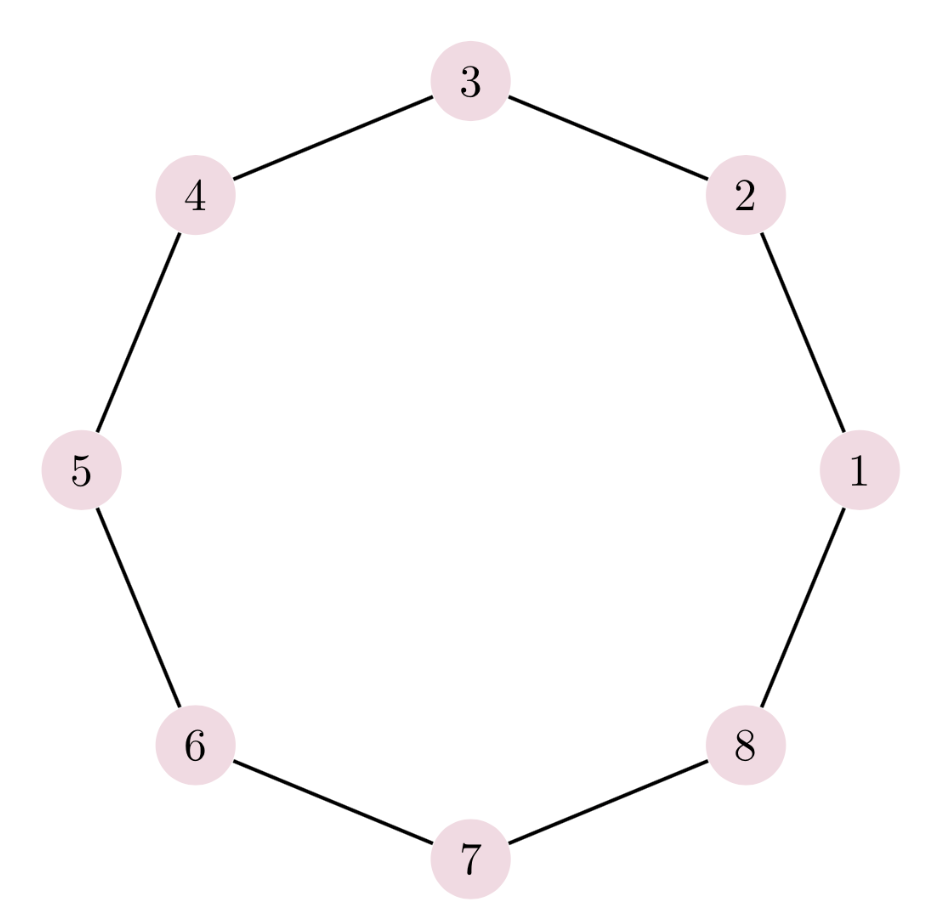
\includegraphics[width=\linewidth]{img/Qiskit/ContQuantumWalk/Graphs/graph0.png}
    \caption{$G_1$}
  \end{subfigure}
  %\hfill
  \begin{subfigure}[t]{.23\textwidth}
    \centering
    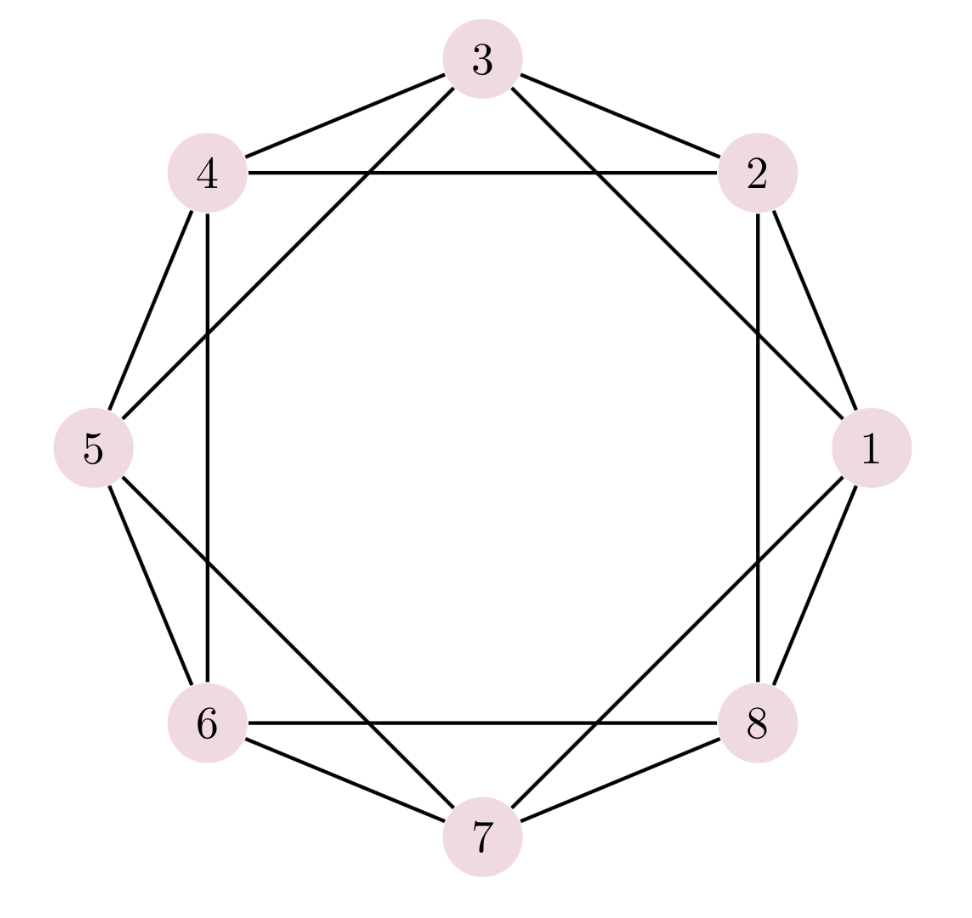
\includegraphics[width=\linewidth]{img/Qiskit/ContQuantumWalk/Graphs/graph1.png}
    \caption{$G_2$}
  \end{subfigure}
  %  \medskip
  \begin{subfigure}[t]{.23\textwidth}
    \centering
    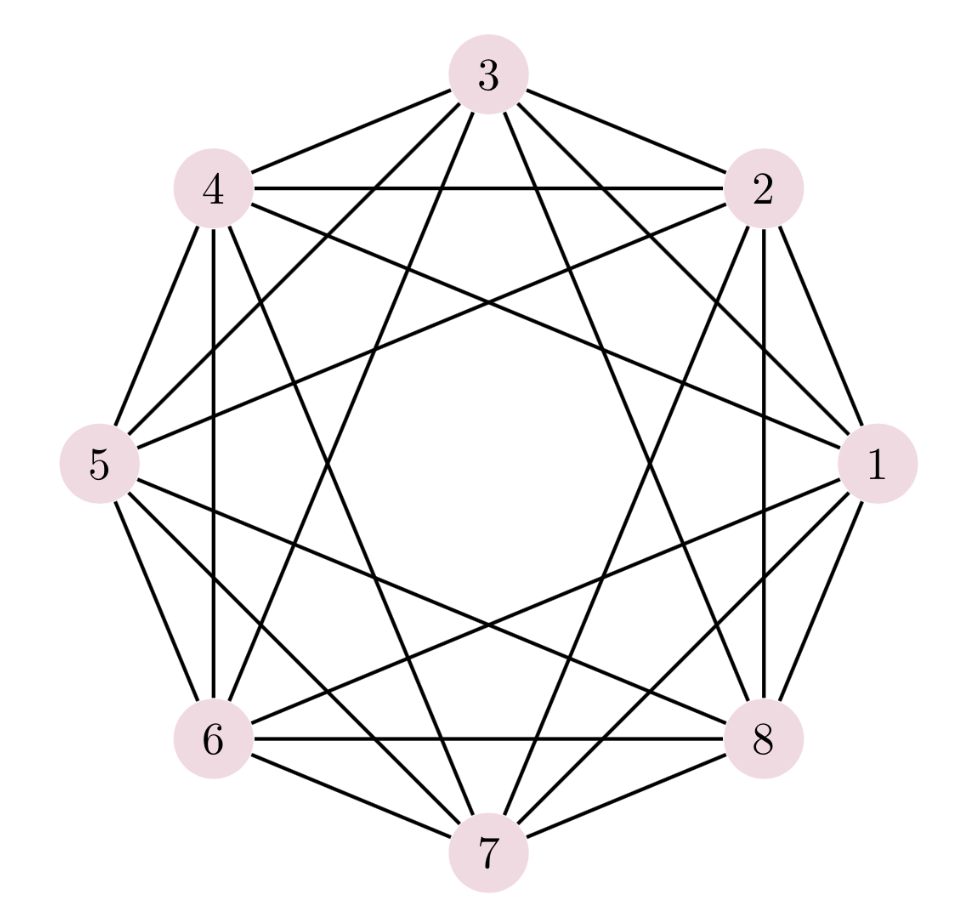
\includegraphics[width=\linewidth]{img/Qiskit/ContQuantumWalk/Graphs/graph2.png}
    \caption{$G_3$}
  \end{subfigure}
  %\hfill
  \begin{subfigure}[t]{.23\textwidth}
    \centering
    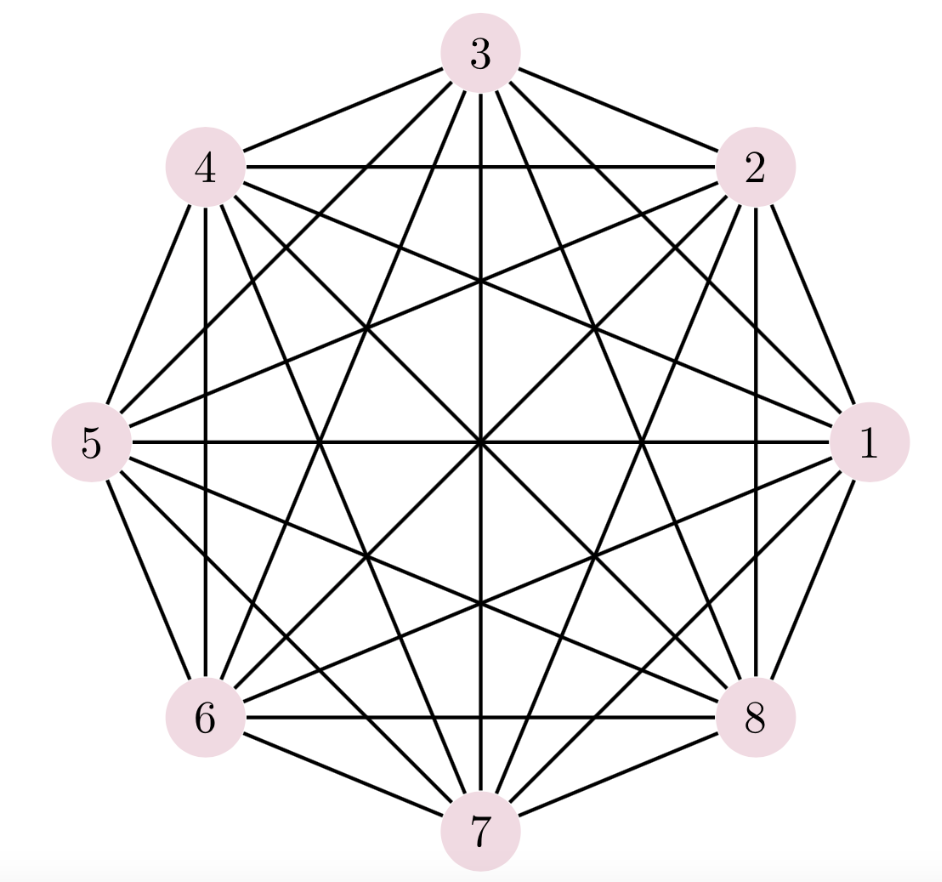
\includegraphics[width=\linewidth]{img/Qiskit/ContQuantumWalk/Graphs/graph3.png}
    \caption{$G_4$}
  \end{subfigure}
  \caption{Circulant graphs $G_k$ for $N=8$ elements.}
  \label{fig:circulantGraphs}
\end{figure}\par

Starting with a smaller $N = 2^2 = 4$ case, two non-isomorphic circulant
graphs can be built. $G_1$ corresponds to the cycle graph, and
$G_2$ to the complete graph. Table \ref{tab:N2TRT} shows the achieved average
fidelities, which were calculated with equation \eqref{eq:avgFid}. Comparing to
the complete graph case presented in \cite{qiang2016}, where a
fidelity of $0.967 \pm 0.003$ was obtained, it is possible to see that the implementation
presented here slightly outperforms it in terms of fidelity.
\begin{table}[!h]
\centering
\begin{tabular}{| l | l | l |}
\hline
m$\setminus G$ & $G_1$               & $G_2$  \\ \hline
0   & 0.98 $\pm$ 0.01 & 0.99 $\pm$ 0.01  \\\hline
1   & 0.98 $\pm$ 0.02 & 0.993 $\pm$ 0.006   \\\hline
\end{tabular}
\caption{Fidelity of quantum state with N=4, backend \textit{Toronto}, and t=1.}
\label{tab:N2TRT}
\end{table}\par

For the $N = 2^3 = 8$ case, table \ref{tab:N3TRT} shows that state fidelity is
greater as graph connectivity increases, and as $m$ increases. This is due to
the fact that a greater $m$ implies a smaller circuit, but also an increase in
error. However, graphs have less distinct eigenvalues as they are more
connected, which means that a higher degree of approximation of the QFT will
generally introduce less errors, while keeping the circuit depth
lower.
\begin{table}[!h]
\centering
%\resizebox{200pt}{30pt}{
\begin{tabular}{| l | l | l | l | l |}
\hline
m$\setminus G$ & $G_1$                & $G_2$                & $G_3$                & $G_4$    \\\hline
0   & 0.80 $\pm$ 0.01 & 0.92 $\pm$ 0.02     & 0.968 $\pm$ 0.007  & 0.965 $\pm$ 0.006 \\\hline
1   & 0.894 $\pm$ 0.007 & 0.95 $\pm$ 0.01   & 0.98 $\pm$ 0.01    & 0.973 $\pm$ 0.008 \\\hline
2   & 0.852 $\pm$ 0.009 & 0.955 $\pm$ 0.004 & 0.985 $\pm$ 0.003  & 0.990 $\pm$ 0.002 \\\hline
\end{tabular}
%}
\caption{Fidelity of quantum state with N=8, backend \textit{Toronto}, and t=1.}
\label{tab:N3TRT}
\end{table}\par

Finally, table \ref{tab:N4TRT} presents the $N = 2^4 = 16$ case. Here, the
behavior is similar to the previous case up to graph $G_5$, meaning that
higher graph connectivity and larger $m$ will result in higher fidelity.
However, graphs $G_6$, $G_7$ and $G_8$, even though highly connected and
with relatively low depth, present lower fidelity. 
\begin{table}[!h]
\centering
\resizebox{\columnwidth}{35pt}{
\begin{tabular}{|l|l|l|l|l|l|l|l|l|l|}
\hline
m$\setminus G$ & G1               & G2    & G3    & G4 & G5    & G6    & G7    & G8   \\ \hline
0   &   0.47 $\pm$ 0.03   &   0.61 $\pm$ 0.02     &   0.78 $\pm$ 0.02       & 0.86 $\pm$ 0.01 &   0.86 $\pm$ 0.01 &   0.70 $\pm$ 0.04   &   0.54 $\pm$ 0.03 &   0.49 $\pm$ 0.04  \\ \hline
1   & 0.50 $\pm$ 0.03     & 0.63 $\pm$ 0.03        & 0.79 $\pm$ 0.03        & 0.87 $\pm$ 0.02 & 0.85 $\pm$ 0.03 & 0.70 $\pm$ 0.03 & 0.55 $\pm$ 0.05 & 0.50 $\pm$ 0.04  \\ \hline
2   & 0.55 $\pm$ 0.03     & 0.71 $\pm$ 0.03     & 0.83 $\pm$ 0.02     & 0.90 $\pm$ 0.01 & 0.89 $\pm$ 0.02 & 0.75 $\pm$ 0.02 & 0.62 $\pm$ 0.04 & 0.59 $\pm$ 0.06  \\ \hline
3   & 0.60 $\pm$ 0.03     & 0.70 $\pm$ 0.02     & 0.85 $\pm$ 0.01     & 0.92 $\pm$ 0.01 & 0.91 $\pm$ 0.01 & 0.80 $\pm$ 0.03 & 0.71 $\pm$ 0.04 & 0.69 $\pm$ 0.04   \\\hline
\end{tabular}
}
\caption{Fidelity of quantum state with N=16, backend \textit{Toronto}, and t=1.}
\label{tab:N4TRT}
\end{table}
This seems to contradict the results in table \ref{tab:N3TRT}. However this
behavior can be explained due to the fact that the probability distribution of
the dynamics of the walk on these structures is highly concentrated in a small
number for vertices. Considering that the size of the circuit starts to push
the limits of NISQ computers, it is expected that the spreading out of the
probability distribution due to the effects of noise produces a lower
fidelity. Nonetheless, the increase of $m$ still has a positive impact on the
fidelity of these circuits, which means that the reduction in circuit size will
indeed produce better results.
\end{document}
